% \documentclass[12pt]{article}
\documentclass[a4paper, t]{article}
\usepackage{fancyhdr}
\usepackage{graphicx}
\usepackage{hyperref}
\usepackage[a4paper, margin=0.8in]{geometry} % Añadido para ajustar los márgenes
\usepackage{array} % Añadido para ajustar el ancho de las columnas
\usepackage{tabularx} % Añadido para ajustar automáticamente el ancho de la tabla
\usepackage{float} % Añadido para forzar la posición de las tablas

\title{SuperMarket Product Distribution}
\author{
    Max Estrade\thanks{\href{mailto:max.estrade@estudiantat.upc.edu}{max.estrade@estudiantat.upc.edu}} \and
    Victor Diez\thanks{\href{mailto:victor.diez@estudiantat.upc.edu}{victor.diez@estudiantat.upc.edu}} \and
    Victor Llorens\thanks{\href{mailto:victor.llorens@estudiantat.upc.edu}{victor.llorens@estudiantat.upc.edu}} \and
    Sergio Shmyhelskyy Yaskevych\thanks{\href{mailto:sergio.shmyhelskyy@estudiantat.upc.edu}{sergio.shmyhelskyy@estudiantat.upc.edu}}
}

\date{Versió d'Entrega : v2}

\begin{document}

\maketitle

\vspace{1cm}  % Espacio para dar separación

\begin{center}
    \textbf{Identificador d'Equip: 23.2}
\end{center}

\newpage

\tableofcontents

\newpage

\section{Introducció}

Aquest document proporciona una descripció detallada de les classes implementades en el projecte "SuperMarket Product Distribution". 
L'objectiu principal és oferir una visió clara de les funcionalitats i característiques de cada classe, 
així com de les estructures de dades utilitzades. A més, es descriuen els mètodes i operacions disponibles 
per a la gestió de productes, usuaris i distribucions dins del sistema.
\\ \\
\noindent El document està estructurat de la següent manera:
\begin{itemize}
    \item Descripció de les Classes Implementades: Una descripció detallada de cada classe, incloent-hi els seus mètodes i funcionalitats.
    \item Persistència de Dades: Informació sobre com es gestionen i emmagatzemen les dades de persistència del sistema.
    \item Estructura de Dades per Classes: Descripció de les estructures de dades utilitzades per a la gestió de productes, llistes de productes i distribucions.
\end{itemize}

\newpage

\section{Descripció de les Classes Implementades}

A continuació es descriuen les classes implementades per cada membre de l’equip, així com les seves característiques i funcionalitats.

\subsection{Capa de Domini}

\subsubsection{Classe UserManager}
La classe \texttt{UserManager} és un singleton que s'encarrega de gestionar les operacions dels usuaris, com ara el registre, l'inici de sessió i la gestió de dades. Proporciona mètodes per afegir, eliminar i consultar usuaris, així com per gestionar les llistes de productes i distribucions dels usuaris actius.

\begin{itemize}
    \item \textbf{registerUser}
    \begin{itemize}
        \item \textbf{Descripció:} Registra un nou usuari al sistema.
        \item \textbf{Paràmetres:}
        \begin{itemize}
            \item \texttt{username} - el nom d'usuari
            \item \texttt{email} - el correu electrònic
            \item \texttt{password} - la contrasenya
        \end{itemize}
        \item \textbf{Llança:} \texttt{UserException} si el nom d'usuari o el correu electrònic ja estan en ús
    \end{itemize}

    \item \textbf{loginUser}
    \begin{itemize}
        \item \textbf{Descripció:} Inicia sessió amb un usuari existent.
        \item \textbf{Paràmetres:}
        \begin{itemize}
            \item \texttt{userInput} - el nom d'usuari o el correu electrònic
            \item \texttt{password} - la contrasenya
        \end{itemize}
        \item \textbf{Llança:} \texttt{UnauthorizedAccessException} si el nom d'usuari/correu electrònic o la contrasenya són incorrectes
    \end{itemize}

    \item \textbf{logoutUser}
    \begin{itemize}
        \item \textbf{Descripció:} Tanca la sessió de l'usuari actiu.
        \item \textbf{Retorna:} cert si la sessió s'ha tancat correctament, fals en cas contrari
    \end{itemize}

    \item \textbf{deleteUser}
    \begin{itemize}
        \item \textbf{Descripció:} Elimina un usuari pel seu nom d'usuari.
        \item \textbf{Paràmetres:}
        \begin{itemize}
            \item \texttt{username} - el nom d'usuari a eliminar
        \end{itemize}
        \item \textbf{Retorna:} cert si l'usuari s'ha eliminat correctament, fals en cas contrari
    \end{itemize}
\end{itemize}

\subsubsection{Classe UserSet}
La classe \texttt{UserSet} representa un conjunt d'usuaris i proporciona mètodes per gestionar-los. Permet afegir, eliminar i consultar usuaris, així com comprovar l'existència d'usuaris pel seu ID, nom d'usuari o correu electrònic.

\begin{itemize}
    \item \textbf{addUser}
    \begin{itemize}
        \item \textbf{Descripció:} Afegeix un usuari al conjunt.
        \item \textbf{Paràmetres:}
        \begin{itemize}
            \item \texttt{user} - l'usuari a afegir
        \end{itemize}
    \end{itemize}

    \item \textbf{removeUser}
    \begin{itemize}
        \item \textbf{Descripció:} Elimina un usuari del conjunt pel seu ID.
        \item \textbf{Paràmetres:}
        \begin{itemize}
            \item \texttt{userID} - l'ID de l'usuari a eliminar
        \end{itemize}
    \end{itemize}

    \item \textbf{getUser}
    \begin{itemize}
        \item \textbf{Descripció:} Obté un usuari pel seu ID.
        \item \textbf{Paràmetres:}
        \begin{itemize}
            \item \texttt{userID} - l'ID de l'usuari a obtenir
        \end{itemize}
        \item \textbf{Retorna:} l'usuari amb l'ID especificat, o null si no es troba
    \end{itemize}
\end{itemize}

\subsubsection{Classe User}
La classe \texttt{User} representa un usuari del sistema. Gestiona els atributs de l'usuari, com ara el seu ID, nom d'usuari, contrasenya i correu electrònic.

\begin{itemize}
    \item \textbf{getUserID}
    \begin{itemize}
        \item \textbf{Descripció:} Obté l'ID de l'usuari.
        \item \textbf{Retorna:} l'ID de l'usuari
    \end{itemize}

    \item \textbf{getUsername}
    \begin{itemize}
        \item \textbf{Descripció:} Obté el nom d'usuari.
        \item \textbf{Retorna:} el nom d'usuari
    \end{itemize}

    \item \textbf{setUsername}
    \begin{itemize}
        \item \textbf{Descripció:} Estableix el nom d'usuari.
        \item \textbf{Paràmetres:}
        \begin{itemize}
            \item \texttt{username} - el nou nom d'usuari
        \end{itemize}
    \end{itemize}
\end{itemize}

\subsubsection{Classe CurrentUser}
La classe \texttt{CurrentUser} representa l'usuari actualment actiu en el sistema. Gestiona els atributs de l'usuari, així com les seves llistes de productes i distribucions.

\begin{itemize}
    \item \textbf{addProductList}
    \begin{itemize}
        \item \textbf{Descripció:} Afegeix una llista de productes a l'usuari.
        \item \textbf{Paràmetres:}
        \begin{itemize}
            \item \texttt{productListName} - el nom de la llista de productes a afegir
        \end{itemize}
    \end{itemize}

    \item \textbf{removeProductList}
    \begin{itemize}
        \item \textbf{Descripció:} Elimina una llista de productes de l'usuari pel seu nom.
        \item \textbf{Paràmetres:}
        \begin{itemize}
            \item \texttt{productListName} - el nom de la llista de productes a eliminar
        \end{itemize}
    \end{itemize}

    \item \textbf{getUserProductLists}
    \begin{itemize}
        \item \textbf{Descripció:} Obté totes les llistes de productes de l'usuari.
        \item \textbf{Retorna:} un conjunt de totes les llistes de productes
    \end{itemize}
\end{itemize}

\subsubsection{Classe Shelf}
La classe \texttt{Shelf} és una classe que representa una prestatgeria del sistema. 
Conté una matriu de productes que representa la distribució de productes en la prestatgeria. 

Té com atributs id (que és la seva clau primaria), xsize(representa el tamany horizontal de la prestatgeria), ysize (vertical), 
distributionHistory(un historial de les ultime distribusions que s’han fet) i té una relació amb les classes DIstribution.
Quan es crea una instància de \texttt{Shelf}, aquesta es crea buida i es pot anar omplint amb distribucions de productes (que es poden afegir, eliminar, consultar, etc.), 
que inicialment serà generada per un algorisme d’ordenació de productes (\texttt{BruteForceAlgorithm} o \texttt{HillClimbingAlgorithm}). 
És a dir, té una llista de productes associada i una llista de distribucions, on cada distribució és una matriu de productes. 
La distribució actual de la prestatgeria (l’última de la llista de distribucions) es pot consultar en qualsevol moment, i es pot canviar per una altra distribució.

\subsubsection{Classe Similarity}
La classe \texttt{Similarity} és una classe associativa que representa el grau de relació i similitud entre dos productes del sistema, 
de forma que un producte que tingui major similitud amb un altre producte es pugui després tenir en compte per distribuir-los en una prestatgeria. 
És la classe més granular del sistema, ja que representa la relació entre dos productes.

\subsubsection{Classe Product}
La classe \texttt{Product} representa un producte del sistema. Cada producte té un nom, una categoria, un preu (es guarda en tot cas el seu preu original) i una quantitat.
Inclou característiques addicionals com la validació, el seguiment de descomptes i els mètodes d'utilitat.

\subsubsection{Classe ProductList}
La classe \texttt{ProductList} representa una llista de productes del sistema. Cada llista de productes té un nom i una llista de productes associats (usant un diccionari \texttt{Set\textless \textgreater}). 
Aquesta classe permet afegir productes a la llista, eliminar-los, consultar-los, etc. Per dur a terme aquestes operacions, depèn de la classe \texttt{Product}. Cada vegada que es modifica la llista de productes, es guarda un registre de la modificació amb la data i hora en què s’ha fet en el ControllerDomain.

\subsubsection{Classe ProductManager}
La classe \texttt{ProductManager} és un singleton que s’encarrega de gestionar les instàncies de \texttt{Product} del sistema i les seves relacions amb les llistes de productes \texttt{ProductList} .  
S’aplica aquest patró de disseny, de forma que els controladors del domini puguin gestionar correctament les instàncies en el sistema. Gestiona tota mena d’operacions relacionades amb afegir productes,
eliminar-los o consultar-los, juntament amb les múltiples llistes de productes, proporcionant mètodes per afegir, eliminar i editar productes. 
S’encarrega de mantenir un mapa de similituts* entre tots els productes del catàleg i les llistes de productes.  
Per gestionar els productes, fa servir diccionaris per guardar els productes i les llistes amb els seu nom com a clau per poder buscar-los ràpidament de manera eficient.

\begin{itemize}
    \item \textbf{addProductToCatalog}
    \begin{itemize}
        \item \textbf{Descripció:} Afegeix un producte únic al catàleg de productes del supermercat.
        \item \textbf{Paràmetres:}
        \begin{itemize}
            \item \texttt{productName} - el nom del producte
            \item \texttt{category} - la categoria del producte
            \item \texttt{price} - el preu del producte
            \item \texttt{amount} - la quantitat del producte
            \item \texttt{similarities} - una llista de noms de productes i valors de similitud
        \end{itemize}
        \item \textbf{Llança:} \texttt{ProductException} si el producte ja existeix al catàleg
    \end{itemize}

    \item \textbf{removeProductFromCatalog}
    \begin{itemize}
        \item \textbf{Descripció:} Elimina un producte del catàleg.
        \item \textbf{Paràmetres:}
        \begin{itemize}
            \item \texttt{productName} - el nom del producte a eliminar
        \end{itemize}
        \item \textbf{Llança:} \texttt{ProductException} si el producte no existeix al catàleg
    \end{itemize}

    \item \textbf{increaseProductQuantity}
    \begin{itemize}
        \item \textbf{Descripció:} Augmenta la quantitat d'un producte al catàleg.
        \item \textbf{Paràmetres:}
        \begin{itemize}
            \item \texttt{productName} - el nom del producte
            \item \texttt{amount} - la quantitat a augmentar
        \end{itemize}
        \item \textbf{Retorna:} la quantitat restant del producte
        \item \textbf{Llança:} \texttt{ProductException} si el producte no existeix o la quantitat no és positiva
    \end{itemize}

    \item \textbf{decreaseProductQuantity}
    \begin{itemize}
        \item \textbf{Descripció:} Disminueix la quantitat d'un producte al catàleg.
        \item \textbf{Paràmetres:}
        \begin{itemize}
            \item \texttt{productName} - el nom del producte
            \item \texttt{amount} - la quantitat a disminuir
        \end{itemize}
        \item \textbf{Retorna:} la quantitat restant del producte
        \item \textbf{Llança:} \texttt{ProductException} si el producte no existeix, la quantitat no és vàlida o la quantitat resultant és negativa
    \end{itemize}

    \item \textbf{applyDiscountToProduct}
    \begin{itemize}
        \item \textbf{Descripció:} Aplica un descompte a un producte i registra la modificació.
        \item \textbf{Paràmetres:}
        \begin{itemize}
            \item \texttt{productName} - el nom del producte
            \item \texttt{percentage} - el percentatge de descompte a aplicar
        \end{itemize}
        \item \textbf{Llança:} \texttt{ProductException} si el producte no existeix al catàleg
    \end{itemize}

    \item \textbf{createProductList}
    \begin{itemize}
        \item \textbf{Descripció:} Crea una nova llista de productes al supermercat.
        \item \textbf{Paràmetres:}
        \begin{itemize}
            \item \texttt{listName} - el nom de la llista de productes
            \item \texttt{category} - la categoria de la llista de productes
        \end{itemize}
        \item \textbf{Retorna:} cert si la llista s'ha creat, fals si ja existeix
        \item \textbf{Llança:} \texttt{ProductListException} si la llista de productes ja existeix
    \end{itemize}

    \item \textbf{removeProductList}
    \begin{itemize}
        \item \textbf{Descripció:} Elimina una llista de productes del supermercat.
        \item \textbf{Paràmetres:}
        \begin{itemize}
            \item \texttt{listName} - el nom de la llista de productes a eliminar
        \end{itemize}
        \item \textbf{Llança:} \texttt{ProductListException} si la llista de productes no existeix
    \end{itemize}

    \item \textbf{addProductToList}
    \begin{itemize}
        \item \textbf{Descripció:} Afegeix un producte existent del catàleg a una llista de productes específica.
        \item \textbf{Paràmetres:}
        \begin{itemize}
            \item \texttt{listName} - el nom de la llista de productes a la qual s'afegirà el producte
            \item \texttt{productName} - el nom del producte a afegir
        \end{itemize}
        \item \textbf{Llança:} \texttt{ProductListException} si la llista de productes no existeix
        \item \textbf{Llança:} \texttt{ProductException} si el producte no existeix
    \end{itemize}

    \item \textbf{removeProductFromList}
    \begin{itemize}
        \item \textbf{Descripció:} Elimina un producte d'una llista de productes especificada.
        \item \textbf{Paràmetres:}
        \begin{itemize}
            \item \texttt{listName} - el nom de la llista de productes de la qual s'eliminarà el producte
            \item \texttt{productName} - el nom del producte a eliminar de la llista
        \end{itemize}
        \item \textbf{Llança:} \texttt{ProductListException} si la llista de productes no existeix
        \item \textbf{Llança:} \texttt{ProductException} si el producte no existeix a la llista
    \end{itemize}

    \item \textbf{setSimilarity}
    \begin{itemize}
        \item \textbf{Descripció:} Afegeix una similitud entre dos productes.
        \item \textbf{Paràmetres:}
        \begin{itemize}
            \item \texttt{product1} - el nom del primer producte
            \item \texttt{product2} - el nom del segon producte
            \item \texttt{similarity} - el valor de similitud
        \end{itemize}
        \item \textbf{Llança:} \texttt{ProductException} si algun dels productes no existeix
    \end{itemize}
\end{itemize}

*Nota: Respecte a la primera entrega: S’ha deixat d’utilitzar Similarity Manager.

\subsubsection{Classe Distribution}
La classe \texttt{Distribution} representa una distribució de productes en una prestatgeria del sistema. 
Guarda la distribució de productes com una matriu que representa el prestatge de la mateixa manera que la imatge. 
Aquesta classe permet afegir productes a la distribució, eliminar-los, consultar-los, etc.
Conté la data de creació i modificació de la distribució, així com la llista de productes associats a la distribució.

\subsubsection{Classe DistributionManager}
La classe \texttt{DistributionManager} és un singleton que s’encarrega de gestionar les instàncies de \texttt{Distribution} del sistema. 
Permet gestionar més fàcilment les distribucions de productes en les prestatgeries del sistema, podent afegir distribucions,
eliminar-les, modificar-les, consultar-les, etc.
Cada vegada que es modifica una distribució, es guarda un registre de la modificació amb la data i hora en què s’ha fet.

\subsubsection{Classe AbstractAlgorithm}
La classe \texttt{AbstractAlgorithm} és una classe abstracta que conté la funció polimòrfica \texttt{orderProductList}.
Aquesta funció permet ordenar una llista de productes en una prestatgeria, i retorna la distribució de productes ordenada.
Aquesta classe conté també dues funcions comunes a les classes que heretin d’aquesta.

\subsubsection{Classe BruteForceAlgorithm}
La classe \texttt{BruteForceAlgorithm} és una classe que hereta de \texttt{AbstractAlgorithm} i implementa la funció \texttt{orderProductList}.
Implementa un algorisme de força bruta \textit{backtracking} per trobar una distribució de productes ordenada en una prestatgeria.

\subsubsection{Classe HillClimbingAlgorithm}
La classe \texttt{HillClimbingAlgorithm} és una classe que hereta de \texttt{AbstractAlgorithm} i implementa la funció \texttt{orderProductList}.
Implementa un algorisme d’aproximació \textit{Hill Climbing} per trobar una distribució de productes ordenada en una prestatgeria.

\newpage
\subsubsection{Classe InputManager}
La classe \texttt{InputManager} és un singleton que s’encarrega de gestionar les entrades del sistema. 
S’aplica aquest patró de disseny, de forma que els controladors del domini puguin gestionar correctament les entrades en el sistema. 
Gestiona tota mena d’operacions relacionades amb les entrades del sistema, com ara llegir fitxers, escriure fitxers, etc. 
És usada principalment per la classe \texttt{ControllerDomain/DriverControllerDomain} per llegir les dades i comandes d’entrada del sistema.

Permeten l’execució a través d’una sèrie de comandes que es poden llegir des d’un fitxer o des de la consola:

\begin{itemize}
    \item \texttt{CREATE\_LIST listName and listCategory}
    \item \texttt{DELETE\_LIST listId}
    \item \texttt{ADD\_PRODUCT nameProduct and nameList}
    \item \texttt{REMOVE\_PRODUCT nameProduct and nameList}
    \item \texttt{SHOW\_SIMILARITIES nomProduct1, nomProduct2, and newSimilarity}
    \item \texttt{CHANGE\_SIMILARITIES nomProduct1, nomProduct2, and newSimilarity}
    \item \texttt{DECREASE\_PRODUCT\_QUANTITY nameProduct and quantity}
    \item \texttt{INCREASE\_PRODUCT\_QUANTITY nameProduct and quantity}
    \item \texttt{ADD\_PRODUCT\_TO\_CATALOG productName, category, price, and amount}
    \item \texttt{REMOVE\_PRODUCT\_CATALOG productName}
    \item \texttt{SHOW\_MODIFICATION\_LOG}
    \item \texttt{CREATE\_SHELF id, maxCapacity, listName, algorithm}
    \item \texttt{CHANGE\_SHELF\_ALGORITHM shelfId and algorithm}
    \item \texttt{CHANGE\_PRODUCT\_LIST\_AT\_SHELF shelfId and listName}
    \item \texttt{CREATE\_NEW\_DISTRIBUTION\_FILE newName, path, and shelfId}
    \item \texttt{SHOW\_PRODUCTS}
    \item \texttt{SHOW\_ALL\_LISTS}
    \item \texttt{SHOW\_DISTRIBUTION idShelf}
    \item \texttt{CREATE\_DISTRIBUTION idShelf, nomDistribution and (optional) Depth}
    \item \texttt{MODIFY\_DISTRIBUTION nameDistribution, nameProduct1, nameProduct2}
    \item \texttt{SHOW\_SHELVES}
\end{itemize}

\newpage
\subsubsection{Classe ControllerDomain}
La classe \texttt{ControllerDomain} és un singleton que s’encarrega de gestionar les operacions del sistema. 
Aquesta és la classe principal que gestiona la capa de domini del sistema, i s’encarrega de gestionar les 
operacions del sistema cap a les classes del domini i retornar les sortides del sistema cap a la capa de presentació 
(\texttt{Controlador de Presentació}). S’aplica aquest patró de disseny, de forma que els controladors del domini puguin 
gestionar correctament les operacions en el sistema. S’encarrega d’instanciar la resta de controladors, i proporciona una 
interfície més pròxima a l’usuari dels mètodes de la resta de controladors. 
\\ \\
\noindent També es comunica amb la classe \texttt{InputManager} per llegir les dades i comandes d’entrada del sistema. 
Gestiona tota mena d’operacions relacionades amb les operacions del sistema, com ara afegir productes, eliminar-los, consultar-los, etc. 
És usada principalment per la classe \texttt{DriverControllerDomain} per gestionar les operacions del sistema.
\\ \\
\noindent A més, el \texttt{ControllerDomain} també s'encarrega de la gestió dels usuaris i de l'usuari actual del sistema.

\begin{itemize}
    \item \textbf{registerUser}
    \begin{itemize}
        \item \textbf{Descripció:} Registra un nou usuari al sistema.
        \item \textbf{Paràmetres:}
        \begin{itemize}
            \item \texttt{username} - el nom d'usuari
            \item \texttt{email} - el correu electrònic
            \item \texttt{password} - la contrasenya
        \end{itemize}
        \item \textbf{Llança:} \texttt{UserException} si el nom d'usuari o el correu electrònic ja estan en ús
    \end{itemize}

    \item \textbf{loginUser}
    \begin{itemize}
        \item \textbf{Descripció:} Inicia sessió amb un usuari existent.
        \item \textbf{Paràmetres:}
        \begin{itemize}
            \item \texttt{userInput} - el nom d'usuari o el correu electrònic
            \item \texttt{password} - la contrasenya
        \end{itemize}
        \item \textbf{Llança:} \texttt{UnauthorizedAccessException} si el nom d'usuari/correu electrònic o la contrasenya són incorrectes
    \end{itemize}

    \item \textbf{logoutUser}
    \begin{itemize}
        \item \textbf{Descripció:} Tanca la sessió de l'usuari actiu.
        \item \textbf{Retorna:} cert si la sessió s'ha tancat correctament, fals en cas contrari
    \end{itemize}

    \item \textbf{deleteUser}
    \begin{itemize}
        \item \textbf{Descripció:} Elimina un usuari pel seu nom d'usuari.
        \item \textbf{Paràmetres:}
        \begin{itemize}
            \item \texttt{username} - el nom d'usuari a eliminar
        \end{itemize}
        \item \textbf{Retorna:} cert si l'usuari s'ha eliminat correctament, fals en cas contrari
    \end{itemize}

    \item \textbf{addProductToCatalog}
    \begin{itemize}
        \item \textbf{Descripció:} Afegeix un producte únic al catàleg de productes del supermercat.
        \item \textbf{Paràmetres:}
        \begin{itemize}
            \item \texttt{productName} - el nom del producte
            \item \texttt{category} - la categoria del producte
            \item \texttt{price} - el preu del producte
            \item \texttt{amount} - la quantitat del producte
            \item \texttt{similarities} - una llista de noms de productes i valors de similitud
        \end{itemize}
        \item \textbf{Llança:} \texttt{ProductException} si el producte ja existeix al catàleg
    \end{itemize}

    \item \textbf{removeProductFromCatalog}
    \begin{itemize}
        \item \textbf{Descripció:} Elimina un producte del catàleg.
        \item \textbf{Paràmetres:}
        \begin{itemize}
            \item \texttt{productName} - el nom del producte a eliminar
        \end{itemize}
        \item \textbf{Llança:} \texttt{ProductException} si hi ha un error en eliminar el producte del catàleg
    \end{itemize}

    \item \textbf{updateProduct}
    \begin{itemize}
        \item \textbf{Descripció:} Actualitza un producte en el catàleg.
        \item \textbf{Paràmetres:}
        \begin{itemize}
            \item \texttt{name} - el nom del producte
            \item \texttt{category} - la categoria del producte
            \item \texttt{price} - el preu del producte
            \item \texttt{amount} - la quantitat del producte
            \item \texttt{similarities} - una llista de parells amb el nom del producte i el valor de similitud
        \end{itemize}
        \item \textbf{Llança:} \texttt{ProductException} si el nom del producte és invàlid
    \end{itemize}

    \item \textbf{createProductList}
    \begin{itemize}
        \item \textbf{Descripció:} Crea una nova llista de productes amb una categoria especificada.
        \item \textbf{Paràmetres:}
        \begin{itemize}
            \item \texttt{listName} - el nom de la llista de productes
            \item \texttt{category} - la categoria dels productes en la llista
        \end{itemize}
        \item \textbf{Llança:} \texttt{ProductListException} si el nom de la llista és invàlid
    \end{itemize}

    \item \textbf{addProductToList}
    \begin{itemize}
        \item \textbf{Descripció:} Afegeix un producte a una llista especificada.
        \item \textbf{Paràmetres:}
        \begin{itemize}
            \item \texttt{productName} - el nom del producte a afegir a la llista
            \item \texttt{listName} - el nom de la llista a la qual s'afegirà el producte
        \end{itemize}
        \item \textbf{Llança:} \texttt{ProductException} si hi ha un error en afegir el producte a la llista
        \item \textbf{Llança:} \texttt{ProductListException} si hi ha un problema amb la llista de productes especificada
    \end{itemize}

    \item \textbf{removeProductFromList}
    \begin{itemize}
        \item \textbf{Descripció:} Elimina un producte d'una llista específica.
        \item \textbf{Paràmetres:}
        \begin{itemize}
            \item \texttt{productName} - el nom del producte
            \item \texttt{listName} - el nom de la llista de productes
        \end{itemize}
        \item \textbf{Llança:} \texttt{ProductException} si el nom del producte és invàlid
        \item \textbf{Llança:} \texttt{ProductListException} si el nom de la llista és invàlid
    \end{itemize}

    \item \textbf{decreaseProductQuantity}
    \begin{itemize}
        \item \textbf{Descripció:} Disminueix la quantitat d'un producte especificat en el catàleg.
        \item \textbf{Paràmetres:}
        \begin{itemize}
            \item \texttt{productName} - el nom del producte la quantitat del qual es disminuirà
            \item \texttt{quantity} - la quantitat en què es reduirà la quantitat del producte
        \end{itemize}
        \item \textbf{Llança:} \texttt{ProductException} si hi ha un error en disminuir la quantitat del producte
    \end{itemize}

    \item \textbf{increaseProductQuantity}
    \begin{itemize}
        \item \textbf{Descripció:} Augmenta la quantitat d'un producte especificat en el catàleg.
        \item \textbf{Paràmetres:}
        \begin{itemize}
            \item \texttt{productName} - el nom del producte la quantitat del qual s'augmentarà
            \item \texttt{quantity} - la quantitat en què s'augmentarà la quantitat del producte
        \end{itemize}
        \item \textbf{Llança:} \texttt{ProductException} si hi ha un error en augmentar la quantitat del producte
    \end{itemize}

    \item \textbf{applyDiscountToList}
    \begin{itemize}
        \item \textbf{Descripció:} Aplica un descompte a tots els productes d'una llista de productes especificada.
        \item \textbf{Paràmetres:}
        \begin{itemize}
            \item \texttt{listName} - el nom de la llista de productes a la qual s'aplicarà el descompte
            \item \texttt{percentage} - el percentatge de descompte a aplicar als productes de la llista
        \end{itemize}
        \item \textbf{Llança:} \texttt{ProductListException} si hi ha un error en aplicar el descompte a la llista de productes
    \end{itemize}

    \item \textbf{createShelf}
    \begin{itemize}
        \item \textbf{Descripció:} Crea una nova prestatgeria amb la capacitat, llista de productes i algorisme especificats.
        \item \textbf{Paràmetres:}
        \begin{itemize}
            \item \texttt{id} - l'identificador únic de la prestatgeria
            \item \texttt{xcapacity} - la capacitat en l'eix x (amplada) de la prestatgeria
            \item \texttt{ycapacity} - la capacitat en l'eix y (alçada) de la prestatgeria
            \item \texttt{listName} - el nom de la llista de productes a associar amb la prestatgeria
            \item \texttt{algorithm} - l'algorisme a utilitzar per a l'ordenació de productes (1 per Força Bruta, 2 per Hill Climbing)
        \end{itemize}
        \item \textbf{Llança:} \texttt{ShelfException} si l'identificador de la prestatgeria ja existeix, o si hi ha un algorisme invàlid, o una capacitat de prestatgeria invàlida
        \item \textbf{Llança:} \texttt{ProductListException} si la llista de productes està buida, o si la llista de productes no cap a la prestatgeria a causa de la seva mida
    \end{itemize}

    \item \textbf{changeProductListAtShelf}
    \begin{itemize}
        \item \textbf{Descripció:} Canvia la llista de productes associada a una prestatgeria especificada.
        \item \textbf{Paràmetres:}
        \begin{itemize}
            \item \texttt{idShelf} - l'identificador de la prestatgeria la llista de productes de la qual es canviarà
            \item \texttt{listName} - el nom de la nova llista de productes a assignar a la prestatgeria
        \end{itemize}
        \item \textbf{Llança:} \texttt{ShelfException} si la prestatgeria amb l'identificador especificat no existeix
        \item \textbf{Llança:} \texttt{ProductListException} si la nova llista de productes excedeix la capacitat de la prestatgeria
    \end{itemize}

    \item \textbf{changeShelfAlgorithm}
    \begin{itemize}
        \item \textbf{Descripció:} Canvia l'algorisme utilitzat per a l'ordenació de productes en una prestatgeria especificada.
        \item \textbf{Paràmetres:}
        \begin{itemize}
            \item \texttt{id} - l'identificador de la prestatgeria l'algorisme de la qual es canviarà
            \item \texttt{algorithm} - l'identificador de l'algorisme a aplicar (1 per Força Bruta, 2 per Hill Climbing)
        \end{itemize}
        \item \textbf{Llança:} \texttt{ShelfException} si la prestatgeria amb l'identificador especificat no existeix o si l'identificador de l'algorisme és invàlid
    \end{itemize}

    \item \textbf{createNewDistribution}
    \begin{itemize}
        \item \textbf{Descripció:} Crea una nova distribució per a una prestatgeria especificada.
        \item \textbf{Paràmetres:}
        \begin{itemize}
            \item \texttt{idShelf} - l'identificador de la prestatgeria per a la qual es crearà la distribució
            \item \texttt{nameDistribution} - el nom de la nova distribució
            \item \texttt{limit} - el límit de profunditat per a la distribució (ha de ser superior a 0)
        \end{itemize}
        \item \textbf{Llança:} \texttt{ShelfException} si la prestatgeria especificada no existeix
        \item \textbf{Llança:} \texttt{DistributionException} si el límit de profunditat és invàlid (és a dir, zero o negatiu)
    \end{itemize}

    \item \textbf{deleteShelf}
    \begin{itemize}
        \item \textbf{Descripció:} Elimina una prestatgeria del mapa de prestatgeries pel seu identificador.
        \item \textbf{Paràmetres:}
        \begin{itemize}
            \item \texttt{id} - l'identificador únic de la prestatgeria a eliminar
        \end{itemize}
        \item \textbf{Llança:} \texttt{ShelfException} si la prestatgeria amb l'identificador especificat no existeix
    \end{itemize}
\end{itemize}

\newpage
\subsection{Capa de Persistència}

\subsubsection{Classe ControllerPersistence} La classe \texttt{ControllerPersistence} és un singleton que s'encarrega de gestionar les operacions de persistència del sistema. Proporciona mètodes per carregar i guardar dades de productes, usuaris i distribucions.  \begin{itemize} \item \textbf{loadProductCatalog} \begin{itemize} \item \textbf{Descripció:} Carrega el catàleg de productes des del fitxer de configuració. \item \textbf{Retorna:} el catàleg de productes carregat \end{itemize}
\item \textbf{saveProductCatalog}
\begin{itemize}
    \item \textbf{Descripció:} Desa el catàleg de productes al fitxer de configuració.
\end{itemize}

\item \textbf{loadUserCredentials}
\begin{itemize}
    \item \textbf{Descripció:} Carrega les credencials dels usuaris des del fitxer de configuració.
    \item \textbf{Retorna:} un conjunt d'usuaris carregat
\end{itemize}

\item \textbf{saveUserCredentials}
\begin{itemize}
    \item \textbf{Descripció:} Desa les credencials dels usuaris al fitxer de configuració.
\end{itemize}

\item \textbf{loadUserDistributions}
\begin{itemize}
    \item \textbf{Descripció:} Carrega les distribucions d'un usuari des del directori de l'usuari.
    \item \textbf{Paràmetres:}
    \begin{itemize}
        \item \texttt{username} - el nom d'usuari
    \end{itemize}
    \item \textbf{Retorna:} un mapa de distribucions carregat
\end{itemize}

\item \textbf{saveUserDistributions}
\begin{itemize}
    \item \textbf{Descripció:} Desa les distribucions d'un usuari al directori de l'usuari.
    \item \textbf{Paràmetres:}
    \begin{itemize}
        \item \texttt{username} - el nom d'usuari
        \item \texttt{distributions} - la llista de distribucions a desar
    \end{itemize}
\end{itemize}
\end{itemize}

\newpage
\subsubsection{Classe ProductManagerData} La classe \texttt{ProductManagerData} és responsable de gestionar les dades del catàleg de productes. Proporciona mètodes per carregar, desar i inicialitzar el catàleg de productes.  \begin{itemize} \item \textbf{initConfigFile} \begin{itemize} \item \textbf{Descripció:} Inicialitza el fitxer de configuració. Crea el fitxer de configuració si no existeix. \end{itemize}
\item \textbf{loadProductCatalog}
\begin{itemize}
    \item \textbf{Descripció:} Carrega el catàleg de productes des del fitxer.
    \item \textbf{Retorna:} el catàleg de productes carregat
\end{itemize}

\item \textbf{saveProductCatalog}
\begin{itemize}
    \item \textbf{Descripció:} Desa el catàleg de productes i les similituds al fitxer.
\end{itemize}

\item \textbf{getProductCatalog}
\begin{itemize}
    \item \textbf{Descripció:} Obté el catàleg de productes.
    \item \textbf{Retorna:} el catàleg de productes
\end{itemize}

\item \textbf{getProductSimilarities}
\begin{itemize}
    \item \textbf{Descripció:} Obté les similituds dels productes.
    \item \textbf{Retorna:} el mapa de similituds dels productes
\end{itemize}

\item \textbf{getProduct}
\begin{itemize}
    \item \textbf{Descripció:} Recupera un producte del catàleg pel seu nom.
    \item \textbf{Paràmetres:}
    \begin{itemize}
        \item \texttt{productName} - el nom del producte a recuperar
    \end{itemize}
    \item \textbf{Retorna:} el producte amb el nom especificat, o null si no es troba
\end{itemize}
\end{itemize}

\newpage
\subsubsection{Classe UserManagerData} La classe \texttt{UserManagerData} és responsable de gestionar les dades de les credencials dels usuaris. Proporciona mètodes per carregar, desar i verificar les credencials dels usuaris, així com per gestionar les llistes de productes i distribucions específiques dels usuaris.  \begin{itemize} \item \textbf{initConfigFile} \begin{itemize} \item \textbf{Descripció:} Inicialitza el fitxer de configuració. Crea el fitxer de configuració si no existeix. \end{itemize}
\item \textbf{saveUserCredentials}
\begin{itemize}
    \item \textbf{Descripció:} Desa les credencials dels usuaris al fitxer de configuració.
\end{itemize}

\item \textbf{saveUserDistributions}
\begin{itemize}
    \item \textbf{Descripció:} Desa les distribucions d'un usuari al directori de l'usuari.
    \item \textbf{Paràmetres:}
    \begin{itemize}
        \item \texttt{username} - el nom d'usuari
        \item \texttt{distributions} - la llista de distribucions a desar
    \end{itemize}
\end{itemize}

\item \textbf{saveUserProductLists}
\begin{itemize}
    \item \textbf{Descripció:} Desa les llistes de productes d'un usuari al directori de l'usuari.
    \item \textbf{Paràmetres:}
    \begin{itemize}
        \item \texttt{username} - el nom d'usuari
        \item \texttt{productLists} - el mapa de llistes de productes a desar
    \end{itemize}
\end{itemize}

\item \textbf{loadUserCredentials}
\begin{itemize}
    \item \textbf{Descripció:} Carrega les credencials dels usuaris des del fitxer de configuració.
    \item \textbf{Retorna:} un conjunt d'usuaris carregat
\end{itemize}

\item \textbf{loadUserProductLists}
\begin{itemize}
    \item \textbf{Descripció:} Carrega les llistes de productes d'un usuari des del directori especificat.
    \item \textbf{Paràmetres:}
    \begin{itemize}
        \item \texttt{username} - el nom d'usuari
    \end{itemize}
    \item \textbf{Retorna:} un mapa de llistes de productes carregat
\end{itemize}

\item \textbf{loadUserDistributions}
\begin{itemize}
    \item \textbf{Descripció:} Carrega les distribucions d'un usuari des del directori especificat.
    \item \textbf{Paràmetres:}
    \begin{itemize}
        \item \texttt{username} - el nom d'usuari
    \end{itemize}
    \item \textbf{Retorna:} un mapa de distribucions carregat
\end{itemize}

\item \textbf{registerUser}
\begin{itemize}
    \item \textbf{Descripció:} Registra un nou usuari al sistema.
    \item \textbf{Paràmetres:}
    \begin{itemize}
        \item \texttt{username} - el nom d'usuari
        \item \texttt{email} - el correu electrònic
        \item \texttt{hashedPassword} - la contrasenya encriptada
    \end{itemize}
\end{itemize}
\end{itemize}

\newpage

\subsection{Capa de Presentació}

La capa de presentació està formada per vistes, gestionades per un únic controlador de presentació 
que s’encarrega de gestionar les vistes i fer crides al controlador de domini per tenir-ho tot a punt.

\subsubsection{Classe PresentationController}
La classe \texttt{PresentationController} és un singleton que s'encarrega de gestionar la capa de presentació de l'aplicació. 
Proporciona mètodes per interactuar amb les vistes i delega les operacions al controlador de domini.
\\ \\
\noindent Les operacions més destacables són, la de canvi de vistes, les d’omplir les llistes de les vistes, 
i operacions per operacions del controlador de domini (entre elles, getters i setters) per tal de
reduir l’acoblament entre vistes i el controlador de domini (capa de domini) 
i les operacions que creen una vista auxiliar per mostrar a l’usuari informació addicional o errors.
\\ \\
\noindent Les vistes consisteixen en una sèrie de finestres que mostren la informació de l'aplicació a l'usuari,
on principalment es mostren llistes de productes, llistes de distribucions, i llistes de prestatgeries.
Es criden prement botons, permetent navegar per l'aplicació. A més, permeten a l'usuari interactuar amb l'aplicació
mitjançant la introducció de dades i la realització d'operacions.

\section{Persistència de Dades}

Les dades de persistència es guarden en els següents fitxers i directoris:

\begin{itemize}
    \item \textbf{Catàleg de Productes:}
    \begin{itemize}
        \item Fitxer: \texttt{src/main/resources/catalog/products\_catalog.txt}
        \item Descripció: Aquest fitxer conté el catàleg de productes i les seves similituds.
        \item Format:
        \begin{itemize}
            \item Cada línia representa un producte o una similitud entre productes.
            \item Les línies que representen productes tenen el format: \texttt{ProductName,Category,Price,Amount}
            \item Les línies que representen similituds tenen el format: \texttt{Product1,Product2,SimilarityScore}
        \end{itemize}
    \end{itemize}
    \item \textbf{Credencials d'Usuaris:}
    \begin{itemize}
        \item Fitxer: \texttt{src/main/resources/config/user\_credentials.txt}
        \item Descripció: Aquest fitxer conté les credencials dels usuaris registrats.
        \item Format:
        \begin{itemize}
            \item Cada línia representa un usuari.
            \item El format de cada línia és: \texttt{username:email:hashedPassword}
        \end{itemize}
    \end{itemize}
    \item \textbf{Dades d'Usuaris:}
    \begin{itemize}
        \item Directori: \texttt{src/main/resources/users/}
        \item Descripció: Aquest directori conté subdirectoris per a cada usuari, on es guarden les seves llistes de productes i distribucions.
        \begin{itemize}
            \item \texttt{productLists/}: Conté les llistes de productes de l'usuari.
            \begin{itemize}
                \item Format:
                \begin{itemize}
                    \item La primera línia conté el nom de la llista.
                    \item La segona línia conté la categoria de la llista.
                    \item La tercera línia conté la data de l'última modificació.
                    \item Les línies següents contenen els noms dels productes.
                \end{itemize}
            \end{itemize}
            \item \texttt{distributions/}: Conté les distribucions de productes de l'usuari.
        \end{itemize}
    \end{itemize}
\end{itemize}

\newpage
\section{Estructura de Dades per Classes}

\subsection{UserManager}
\begin{itemize}
    \item \textbf{UserSet userSet}:
    \begin{itemize}
        \item Representa el conjunt d'usuaris del sistema.
        \item Guardem els usuaris en un conjunt per poder gestionar-los fàcilment.
        \item Cost d’accedir a un usuari concret: O(1).
        \item Cost d’afegir un usuari: O(1).
        \item Cost d’eliminar un usuari: O(1).
        \item Cost d’accedir a tots els usuaris: O(n).
    \end{itemize}
    \item \textbf{CurrentUser activeUser}:
    \begin{itemize}
        \item Representa l'usuari actualment actiu en el sistema.
        \item Guardem l'usuari actiu per poder gestionar les seves operacions.
        \item Cost d’accedir a l'usuari actiu: O(1).
        \item Cost d’actualitzar l'usuari actiu: O(1).
    \end{itemize}
\end{itemize}

\subsection{UserSet}
\begin{itemize}
    \item \textbf{Map\textless Integer, User\textgreater}:
    \begin{itemize}
        \item Representa el conjunt d'usuaris amb el seu ID com a clau (resultant de la funció de hash del username i correu electrònic).
        \item Guardem els usuaris amb el seu ID com a clau per poder buscar-los ràpidament.
        \item Cost d’accedir a un usuari concret: O(1).
    \end{itemize}
    \item \textbf{Map\textless String, User\textgreater}:
    \begin{itemize}
        \item Representa el conjunt d'usuaris amb el seu nom d'usuari com a clau.
        \item Guardem els usuaris amb el seu nom d'usuari com a clau per poder buscar-los ràpidament.
        \item Cost d’accedir a un usuari concret: O(1).
    \end{itemize}
    \item \textbf{Map\textless String, User\textgreater}:
    \begin{itemize}
        \item Representa el conjunt d'usuaris amb la combinació del seu nom d'usuari i correu electrònic com a clau.
        \item Guardem els usuaris amb la combinació del seu nom d'usuari i correu electrònic com a clau per poder buscar-los ràpidament.
        \item Cost d’accedir a un usuari concret: O(1).
    \end{itemize}
\end{itemize}

\subsection{ProductManager}
\begin{itemize}
    \item \textbf{Map\textless String, Product\textgreater}: 
    \begin{itemize}
        \item Representa el catàleg de productes que tenim a la botiga (registre de productes en sistema).
        \item Guardem els productes amb el seu nom com a clau per poder buscar-los ràpidament.
        \item Cost d’accedir a un producte concret: O(1).
    \end{itemize}
    \item \textbf{Map\textless String, ProductList\textgreater}: 
    \begin{itemize}
        \item Representa les seccions del catàleg com a llistes de productes que tenim a la botiga.
        \item Poden ser llistes buides o amb productes. Només es poden afegir productes que ja existeixen al catàleg.
        \item Guardem les llistes amb el seu nom com a clau per poder buscar-les ràpidament.
        \item Cost d’accedir a una llista concreta: O(1).
    \end{itemize}
    \item \textbf{Map\textless String, Map\textless String, Double\textgreater\textgreater}: 
    \begin{itemize}
        \item Representa les similituds entre productes del catàleg: per cada producte guardem les similituds amb la resta de productes.
        \item Guardem les similituds amb el nom dels dos productes com a clau per poder buscar-les ràpidament.
        \item Cost d’accedir a accedir a un producte concret: O(1).
        \item Cost d’accedir a una similitud concreta: O(1).
    \end{itemize}
\end{itemize}

\subsection{ProductList}
\begin{itemize}
    \item \textbf{Set\textless Product\textgreater}: 
    \begin{itemize}
        \item Representa la llista de productes que tenim a la botiga.
        \item No podem tenir productes repetits a la mateixa llista, per això hem escollit un Set.
        \item Guardem els productes amb el seu nom com a clau per poder buscar-los ràpidament.
        \item Cost d’accedir a un producte concret: O(1).
        \item Cost d’afegir un producte: O(1).
        \item Cost d’eliminar un producte: O(1).
        \item Cost d’actualitzar un producte: O(1).
        \item Cost d’accedir a tots els productes: O(n).
        \item Cost d’accedir a tots els productes d’una categoria: O(n).
    \end{itemize}
\end{itemize}

\subsection{Distribution}
\begin{itemize}
    \item \textbf{ArrayList\textless ArrayList\textless Product\textgreater \textgreater}: 
    \begin{itemize}
        \item Guardem la distribució de productes com una matriu que representa el prestatge.
        \item La mida de la matriu és variable, depenent de la mida de la prestatgeria (xsize, ysize).
    \end{itemize}
\end{itemize}

\newpage
\subsection{ControllerDomain}
\begin{itemize}
    \item \textbf{HashMap\textless int, Shelf\textgreater}: 
    \begin{itemize}
        \item HashMap de Prestatgeries on la clau és la id d’una prestatgeria i el contingut és la prestatgeria.
        \item Guardem les prestatgeries amb la seva id com a clau per poder buscar-les ràpidament.
        \item Cost d’accedir a una prestatgeria concreta: O(1).
        \item Cost d’afegir una prestatgeria: O(1).
        \item Cost d’eliminar una prestatgeria: O(1).
        \item Cost d’actualitzar una prestatgeria: O(1).
        \item Cost d’accedir a totes les prestatgeries: O(n).
        \item Cost d’accedir a totes les prestatgeries amb un algorisme concret: O(n).
        \item Cost d’accedir a totes les prestatgeries amb una llista de productes concreta: O(n).
    \end{itemize}

    \item \textbf{TreeMap\textless LocalDateTime, String \textgreater}:
    \begin{itemize}
        \item S'ha escollit un TreeMap perquè ens permet tenir les modificacions ordenades per data i hora, segons l'ordre natural de les dates.
        \item Guardem un registre de les modificacions que s’han fet al sistema amb la data i hora en què s’han fet.
        \item Guardem el nom de la modificació com a clau i la data i hora com a valor.
        \item Ens permet tenir un registre de les modificacions que s’han fet al sistema.
        \item Cost d’accedir a una modificació concreta: O(log n).
        \item Cost d’afegir una modificació: O(log n).
        \item Cost d’eliminar una modificació: O(log n).
        \item Cost d’actualitzar una modificació: O(log n).
        \item Cost d’accedir a totes les modificacions: O(n).
    \end{itemize}
\end{itemize}

\newpage
\subsection{Algorismes}
\begin{itemize}
    \item \textbf{ArrayList\textless ArrayList\textless Product\textgreater}: 
    \begin{itemize}
        \item És com s’espera que es retorni la distribució ordenada. És una matriu de productes de mida variable. 
        \item Encara que fem els algorismes amb altres estructures, vam decidir retornar-ho amb aquesta per poder representar-la millor per pantalla ja que aquesta estructura de dades es similar a la forma que tindria una prestatgeria a la vida real.  
        \item La distribució esta ordenada com a la imatge.
        \begin{figure}[H]
            \centering
            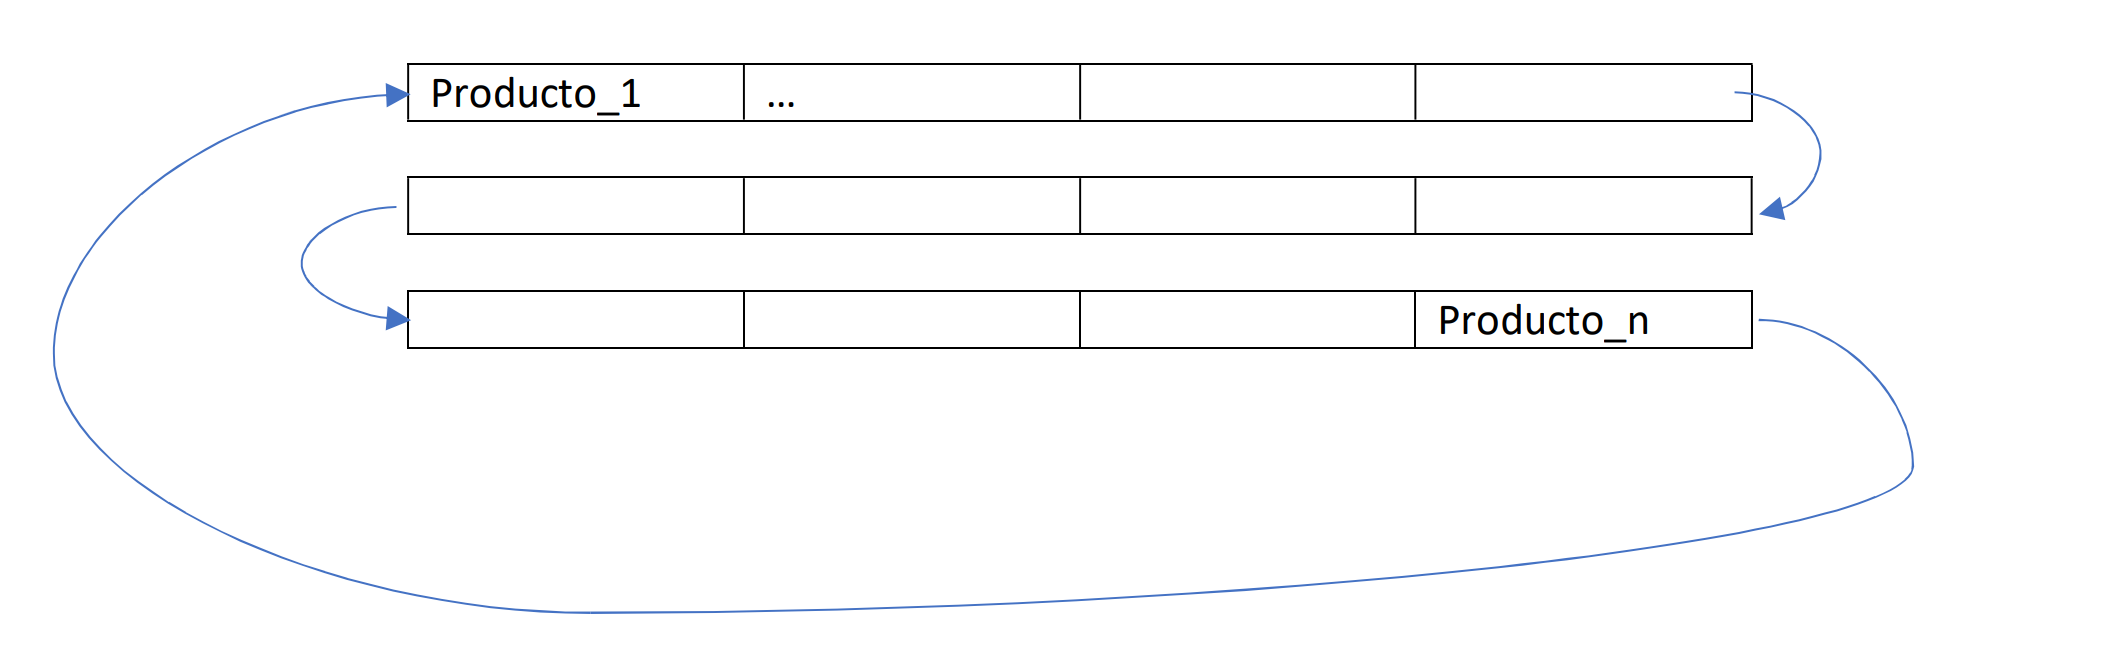
\includegraphics[width=\textwidth]{img/DistributionShelf.png}
            \caption{Distribució de Productes en una Prestatgeria}
            \label{fig:distributionshelf}
        \end{figure}
    \end{itemize}
     \item \textbf{Hashmap\textless String, Pair\textless Integer, Integer\textgreater \textgreater}: 
    \begin{itemize}
        \item A aquest tipus de estructura de dades guardem les coordenades dels productes de la distribució. La clau del mapa es el nom del producte i el seu valor es una parella d’enters que representa les coordenades (x,y) del producte a la matriu. 

        \item Vem decidir afegir aquesta estructura de dades perquè voliem una manera ràpida de trobar els productes a la matriu i un mapa ens permet buscar productes per el seu nom sense tenir que recorrer tota la matriu.
        
        \item Amb aquesta estructura de dades, si volem obtenir la similaritat de 2 productes només hem de fer dos gets, que tenen una complexitat cadascun de O(1). Abans d’aquesta implementació, guardavem la similaritat dels productes com a una llista de similaritats a cada producte amb la relació amb la resta de productes, amb aquesta implementació trobar la similaritat de dos productes tenia una complexitat de O(n).
        
    \end{itemize}
    
     \item \textbf{List\textless Product\textgreater}: 
    \begin{itemize}
        \item Fem servir aquest tipus de dades per crear les distribucions ordenades dins de la classe. Per poder executar els algorismes necesitabem una estructura de dades que ens permeteix canviar l’ordenació dels productes, degut a aquest factor vem descartar estructures de dades com sets o maps. La decisió final va ser entre un vector i una lista, ens vam decantar per la lista.

        \item Com que no és el mateix tipus que el que s’espera retornar tenim una funció privada a la classe AbstractAlgorithm que permet canviar d’aquesta estructura de dades a un ArrayList<ArrayList<Product>>.
        
    \end{itemize}

     \item \textbf{HashSet\textless Product\textgreater}: 
    \begin{itemize}
        \item El fem servir per representar els productes que ja han sortit a la distribució i/o no han de sortir. Hem escollit un HashSet perquè així fem que es guardi només una instància de cada producte i també podem buscar si un producte és al set de manera ràpida

        \item Amb el HashSet el temps per trobar si un producte ha sigut usat amb la operació contains() del HashSet es de O(1), mentres que si fessim servir una estructura de dades no ordenada hauriem de recórrer tots els productes usats, això dóna una complexitat de O(n).
        
    \end{itemize}

    \item \textbf{List\textless List\textless Product\textgreater \textgreater}: 
    \begin{itemize}
        \item El fem servir al algorisme de força bruta per emmagatzemar totes les solucions trobades. Cada List<Product> és una solució i vam decidir guardar-les a una llista pero podriem haver fet servir altres estructures de dades, ja que només necessitabem una estructura que pogués guardas les llistes de productes.

    \end{itemize}
\end{itemize}
\newpage

\section{Algorismes}

Volem tenir dues formes (algorismes) diferents d’ordenar les prestatgeries (shelf). Per implementar-ho hem creat una classe, abstracta AbstractAlgorithm, i una subclase d’aquesta per cada algorisme a implementar, BruteForceAlgorithm i HillClimbingAlgorithm.
\\ \\
La classe AbstractAlgorithm conté una funció orderProductList(...), que serà la funció que farà l’ordenació i és sobreescrita en les subclasses de AbstractAlgorithm, i un parell de funcions comunes auxiliars. A la funció orderProductList(...) li passem com a paràmetres, la llista de productes a ordenar, les mides de la prestatgeria, un límit i un mapa de les coordenades dels productes a la prestatgeria. L'atribut de límit serveix per limitar la cerca de la solució, però per calcular els costos dels algorismes no el farem servir, ja que buscarem el cost en el cas pitjor.
\\ \\
El cas pitjor serà quan la mida de la llista de productes sigui igual o menor al nombre de productes que poden haver-hi en aquesta prestatgeria (mida x * mida y).

\subsection{BruteForceAlgorithm}
Aquesta primera implementació es basa en un algorisme de força bruta (cerca exhaustiva), és a dir, l'algorisme calcula totes les possibles ordenacions i un cop les té totes, escull la millor.
\\ \\
La funció orderProductList crida a la funció generateCombinations. Aquesta guarda totes les combinacions i crida a la funció combineHelper que s’encarrega de la part recursiva del backtracking.
\\
La funció combineHelper rep com atributs: la llista de productes, la combinació actual, el conjunt que conté totes les combinacions, el límit i la mida de la prestatgeria.
\\
\noindent La funció té 2 casos base:
\begin{itemize}
    \item El primer mira si la combinació actual té la mida de la prestatgeria, si la té insereix la combinació a la llista de totes les combinacions, si no continua amb el codi.
    \item L’altre cas base mira si el nombre de combinacions creades és igual al límit (si el límit és menor que 0 vol dir que s’executa ignorant els límits), si és igual acaba el backtracking, si no segueix.
\end{itemize}
La resta del codi és un backtracking normal, on es miren totes les combinacions de productes on no hi ha cap repetit.

\subsubsection{Cost de BruteForceAlgorithm}
L'algorisme primer fa operacions d'inicialització, totes de cost O(1) i seguidament calcula totes les possibles combinacions de productes.
\\ \\
El cost de generar totes les combinacions vàlides és de O(n!). 
\\
Els casos base tenen un cost de O(1) per  tant, els ignorem. En el cas recursiu, el primer cop que s’accedeix el bucle farà N iteracions, la segona farà n -1 ja que no pot accedir a l'element que ja hem inserit a la combinació, la següent farà n - 2 iteracions i així fins a omplir la combinació. És a dir el cost és n * (n-1) * (n-2) * …. * 1 = n! .
\\ \\
Un cop tenim totes les combinacions hem de trobar la millor combinació, per això la suma de similituds de totes les combinacions.
\\ \\
La funció encarregada de calcular la suma de les similituds fa el següent: per cada element de la combinació, obté aquest producte i el següent de la combinació, obté la seva similitud i se la suma al total.
\\
El cost d’obtenir cada producte és O(1), ja que accedeix directament a la memòria. El cost d’obtenir la similitud entre dos productes és O(1),  pel fet que fem servir el mapa de  similituds del producte. Per tant, el cost de calcular la suma de similituds és O(n*O(1)) = O(n).
\\ \\
En conseqüència, el cost de trobar la millor combinació del conjunt de mida n! és O(n * n!). Finalment, es crida la funció adaptToShelf que té de cost O(n). Amb tot això tenim el cost total de la funció orderProductList amb l’algorisme de força bruta, que és O(1+n!+n * n! + n) = O(n * n!)

\newpage
\subsubsection{Pseudocodi de BruteForceAlgorithm}
\begin{verbatim}
funció ordenarLlistaProductes(llista, xsize, ysize, limit, coordenades):
    productes ← convertir a llista els productes de llista
    si productes està buida:
        llençar excepció "Llista buida"

    maxMida ← xsize * ysize
    combinacions ← generarCombinacions(productes, maxMida, limit)
    millor ← llista buida
    maxSimilitud ← 0

    per cada combinació en combinacions:
        suma ← calcularSuma(combinació)
        si suma > maxSimilitud:
            maxSimilitud ← suma
            millor ← combinació

    retornar adaptarADistribució(millor, xsize, ysize, coordenades)

funció generarCombinacions(productes, mida, limit):
    usats ← conjunt buit
    combinacions ← llista buida
    helperCombinacions(productes, mida, 0, llista buida, combinacions, usats, limit)
    retornar combinacions

funció helperCombinacions(productes, mida, inici, combinacióActual, combinacions, usats, limit):
    si mida(combinacióActual) = mínim(mida, mida(productes)):
        afegir còpia de combinacióActual a combinacions
        retornar

    si limit > 0 i mida(combinacions) ≥ limit:
        retornar

    per cada producte a productes:
        si producte no és a usats:
            afegir producte a combinacióActual
            afegir producte a usats
            helperCombinacions(productes, mida, inici + 1, 
                                combinacióActual, combinacions, usats, limit)
            eliminar producte de usats
            treure últim element de combinacióActual
\end{verbatim}

\newpage
\subsection{HillClimbingAlgorithm}
La segona implementació busca trobar una solució de manera més ràpida encara que aquesta no sigui perfecta. Per aconseguir-ho hem escollit fer servir un algorisme d’aproximació Hill Climbing. L’algorisme hill climbing parteix d’una solució inicial i després va mirant les solucions properes per trobar la millor de les veïnes.
\\
Per fer la solució inicial s’escull un producte a l'atzar de la llista de productes i crea una distribució inicial respecte d'aquest producte. Com millor sigui la nostra solució inicial millor serà la nostra solució final, per això hem fet una solució tal que si representem la distribució amb un vector l'element [i] serà l'element disponible amb millor compatibilitat amb l’element [i-1].
\\ \\
Un cop tenim la solució inicial, es comença l’algorisme Hill Climbing. La funció hillClimbing té un bucle en el qual es busquen els veïns de la solució actual que acaba quan no es troba un veí millor o quan s’han fet tantes iteracions del bucle com l’atribut límit (si el límit és menor que 0 vol dir que s’executa ignorant els límits).
\\ \\
Per buscar els veïns pròxims tenim l'operació bestNeighbour on trobem els veïns de la solució actual i canvia la solució actual a la millor trobada. Els veïns s'aconsegueixen fent una sèrie de swaps entre els productes de la solució actual, aconseguint una solució pròxima a l'original. Mentre es generen els veïns guardem el millor d’aquests.

\subsubsection{Cost de HillClimbingAlgorithm}
El primer que fem és obtenir un producte aleatori, això ho fem amb la classe Random de java.util, agafem un integer aleatori i obtenim el producte a la posició d’aquest integer de la llista, fer això té cost O(1).
\\ \\
Després generem la solució inicial, que consisteix d’un bucle que es repetirà n cops, que executa la funció mostSimilarP. La funció mostSimilarP recorre tots els elements i mira la seva similitud, això té un cost de O(n) (hem explicat a l'algorisme BruteForce el cost d’aconseguir una similitud). Això ens dona com a resultat que el cost de la funció per obtenir la 
solució inicial és O($n^2$).
\\ \\
Després per fer el hillClimbing es fa un bucle que en pitjor cas direm que fa k iteracions. Dins d’aquest bucle es crida a la funció bestNeighbor, que es pot explicar com un bucle dins d’un altre on a cada iteració es copia la llista (cost O(n)), es fa un swap de dos productes (cost O(1)) i es mira si és la millor solució (cost O(1)). Com a resultat tenim que la funció hillClimbing té un cost de $O(k*O(n*n*(n+1))) = O(k*n^3)$.
\\ \\
 Finalment, es crida la funció adaptToShelf que té de cost O(n). Amb tot això tenim el cost total de la funció orderProductList amb l’algorisme de Hill Climbing, que és $O(1+n^2+k*n^3) = O(k*n^3)$.

\newpage
\subsubsection{Pseudocodi de HillClimbingAlgorithm}
\begin{verbatim}
function orderProductList(llista, xsize, ysize, limit, coordinates):
    if llista és buida:
        llança excepció "Llista buida"

    maxsize ← xsize * ysize
    randP ← selecciona un producte aleatori de la llista
    initialSolution ← iniSolution(maxsize, randP, llista)
    optimizedSolution ← hillClimbing(initialSolution, limit)

    return adaptToShelf(optimizedSolution, xsize, ysize, coordinates)


function iniSolution(size, startProduct, allProducts):
    solution ← [startProduct]
    used ← {startProduct}

    mentre la solution no estigui completa:
        nextProduct ← mostSimilarP(últimProducte a solution, allProducts, used)
        afegeix nextProduct a solution
        marca nextProduct com a utilitzat
    return solution

function hillClimbing(current, limit):
    repetir fins que no hi hagi millores o es compleixi el límit:
        neighbor ← best_neighbor(current)
        if calculaSum(neighbor) > calculaSum(current):
            current ← neighbor
        else:
            break
    return current


function best_neighbor(llista):
    bestSolution ← llista
    for cada parella de productes a llista:
        intercanvia la parella per crear un nou veí
        if calculaSum(neighbor) > calculaSum(bestSolution):
            bestSolution ← neighbor
    return bestSolution
\end{verbatim}

\end{document}